%!Tex Root = ../main.tex
% ./Packete.tex
% ./Design.tex
% ./Deklarationen.tex
% ./Vorbereitung.tex
% ./Aufgabe1.tex
% ./Aufgabe3.tex
% ./Aufgabe4.tex
% ./Appendix.tex

\section{Aufgabe 2}

\setcounter{exercise}{1}

\begin{frame}[allowframebreaks]{Aufgabe \thesection}{Formale Beschreibung von Schaltkreisen}
\begin{solution}
    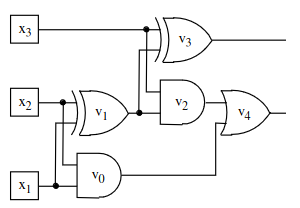
\includegraphics[width=200pt, center]{./figures/Schaltkreis.png}
\end{solution}
\begin{solution}
  \begin{table}
    \centering
    \begin{tblr}{
      cells = {white, c},
      row{1} = {PrimaryColor,fg=white},
      vline{4} = {-}{},
      % hline{2} = {-}{},
    }
      $x_1$&$x_2$&$x_3$&$v_3$&$v_4$\\
      0&0&0&0&0\\
      0&0&1&1&0\\
      0&1&0&1&0\\
      0&1&1&0&1\\
      1&0&0&1&0\\
      1&0&1&0&1\\
      1&1&0&0&1\\
      1&1&1&1&1
    \end{tblr}
  \end{table}
  % \centering
  %   \begin{tabular}{c c c|c c}
  %   \end{tabular}
\end{solution}
\end{frame}
